% !TeX spellcheck = en_GB
%%%%%%%%%%%%%%%%%%%%%%%%%% phdsymp_sample2e.tex %%%%%%%%%%%%%%%%%%%%%%%%%%%%%%
%% changes for phdsymp.cls marked with !PN
%% except all occ. of phdsymp.sty changed phdsymp.cls
%%%%%%%%%%                            %%%%%%%%%%%%%
%%%%%%%%%%  More information: see the header of phdsymp.cls  %%%%%%%%%%%%%
%%%%%%%%%%                            %%%%%%%%%%%%%
%%%%%%%%%%%%%%%%%%%%%%%%%%%%%%%%%%%%%%%%%%%%%%%%%%%%%%%%%%%%%%%%%%%%%%%%%%%%%%%


%\documentclass[10pt]{phdsymp} %!PN
\documentclass[twocolumn]{phdsymp} %!PN
%\documentclass[12pt,draft]{phdsymp} %!PN
%\documentstyle[twocolumn]{phdsymp}
%\documentstyle[12pt,twoside,draft]{phdsymp}
%\documentstyle[9pt,twocolumn,technote,twoside]{phdsymp}

\usepackage[english]{babel}    % Voor nederlandstalige hyphenatie (woordsplitsing)

\usepackage{graphicx}          % Om figuren te kunnen verwerken
\usepackage{graphics}			% Om figuren te verwerken.

\graphicspath{images/}

\usepackage{times}

\hyphenation{}

\def\BibTeX{{\rm B\kern-.05em{\sc i\kern-.025em b}\kern-.08em
  T\kern-.1667em\lower.7ex\hbox{E}\kern-.125emX}}

\newtheorem{theorem}{Theorem}

\begin{document}

\title{The user perceived performance of route planning APIs} %!PN

\author{Bert Marcelis}

\supervisor{Prof. dr. ir. Ruben Verborgh, dr. ing. Pieter Colpaert, Julian Andres Rojas Melendez}

\maketitle

\begin{abstract}

For the Web architectures behind route planning applications, remote procedure calls are commonplace, in which a server calculates the routes for all end-users.
Linked Connections introduces an alternative architecture following the REST constraints, publishing the raw data in fragments.
While benchmarks show a higher cost-efficiency of Linked Connections on the server, it is currently not known how it performs on clients, that now also need to execute the route planning algorithm.
In this work, we study the user-perceived performance of route planning on the client-side, consuming more bandwidth, versus route planning on the server-side. 
An isomorphic app was developed with both route planning on the client-side as on the server-side.
Both technical performance and user-perceived performance were tested among 17 travelers, and 81 respondents gave insights on their use of travel companions.

We found that the performance of Linked Connections heavily depends on the type of information, the query and the user’s device. Linked Connections can be faster or slower than a query answering API based on these parameters. 
The value of offline searches outweighs the slower experience for most users.
For a majority of the users, the benefit of offline searches outweighs the slower speed of Linked Connections. Even though Linked Connections is slower than the reference API, users consider it, on recent devices, as fast as their default application.

\end{abstract}

\begin{keywords}
Linked Connections, public transport
\end{keywords}

\section{Introduction}
\PARstart{P}{ublic} transport is essential in every city. To make use of this transport, travellers frequently use their smartphones or websites to get route planning advice. The most common way to provide these applications and websites with data is by using Remote Procedure Call (RPC) APIs, in which case a server calculates the route or information a user needs, and serves the user with a personalized response. This approach is costly and depends on a continuous connection with the route planning server. Services which need to make queries in bulk, for example to construct insights and collect analytics, use the General Transport Format Specification (GTFS). In this case they can answer all queries themselves, but this method takes too much time and processing power to be applied in mobile end user devices.

Linked Connections tries to find a balance between these two approaches, and has already proven to be 75\% more cost-efficient~\cite{colpaert17}. While the server performance and costs have been researched, the performance and user-experience for a client based on Linked Connections is still unknown. This work will explore various aspects of the performance and user-experience by developing an isomorphic application to compare Linked Connections to a reference RPC API, which uses the same data and algorithms, but runs all calculations on the server. This will show if Linked Connections is a better format -- having a better user-perceived performance and user-experience -- compared to RPC APIs.

\section{State of the art}

Application for public transport are, at this time, commonly driven by RPC APIs. These APIs are based on dumb clients asking a smart server for an answer. On one hand this means it can be used on all clients, as it does not require much resources client-side. On the other hand it can be costly, as every response is personalized, the server has to do processor-intensive tasks and needs to be scaled according to the load. Other negative aspects are the requirements for a constant internet connection, and the fact that individual developers can't alter the route planning algorithm for their application.

When transport data is needed in bulk, for example when someone wants to gather statistics, GTFS can be used. While it is a resource-intensive task to deduce information from GTFS, it does not need API calls for every query. Unfortunately, due to GTFS being resource intensive, it's not fit for mobile devices or cases where results are needed quickly.

Linked connections tries to find a balance between these two technologies, by publishing the raw data in chronological, easy-to-use linked fragments. It's proven to be server efficient, and when load increases, performance increases instead of decreases~\cite{colpaert17}.

\section{User perceived performance of web architectures}

Every web architecture has specific properties, for example latency, performance, cache reuse, ...~\cite{verborgh16}. While these are all technical values, there is also the user-perceived performance. First defined by Roy T. Fielding~\cite{fielding99} as the latency between steady-states for a browser-based application, it comprises all processing needed, not only network traffic. For a (browser) application, the total latency consists of the following parts:
\begin{enumerate}
\item the time needed for the user agent to recognize the event that initiated the action
\item the time required to setup any interaction(s) between components
\item the time required to transmit each interaction to the components
\item the time required to process each interaction on those components
\item the time required to complete sufficient transfer before the user agent is able to begin rendering a usable result.
\item the time required to complete processing of the result of the interaction(s) before the user agent is able to begin rendering a usable result.
\end{enumerate}

While only steps 3,4 and 5 are directly dependent on network connectivity, all of theses steps can be influenced by the used architecture.

When not only focussing on performance, but also on the way users interact with technology, it is important to define the user-experience (UX). UX is a broad term, originally designating the design and usage of interfaces, making it a synonym for interactions and usability~\cite{avila11}, but it is also used for non-instrumental needs and experiences in a more complex way~\cite{avila11}. In this work UX will always be considered in this broader way.

\section{Evaluation design}

In order to evaluate Linked Connections and compare it to RPC APIs, an isomorphic application is developed. This application allows to test Linked Connections and an RPC API, while keeping the user interface and client-side logic identical. An RPC API is developed to be used as a reference for Linked Connections. It is backed by the same data and algorithms as the client-side Linked Connections implementation, thus allowing for a fair comparison. As a result, the only difference is which entity does the processing, and how data is transported.

Using this application, user testing is conducted on 17 test persons. Each tester is asked to search for data he usually searches for, one time using the reference RPC API as data provider, and using the Linked Connections implementation the second time. After testing and grading Linked Connections, they are also encouraged to turn off their network connection and test the offline capabilities using Linked Connections.
Users are only informed over differences between both implementations after the test has completed, as to not bias them. For each implementation, the user grades the speed of listing departures and arrivals for a station (liveboards), journeys from A to B (routes) and vehicle trips (vehicles). Users are also asked to compare each implementation to their currently used application. To conclude, they have to explicitly choose between both implementations regarding speed for each endpoint, and which implementation they favor the most, taking into account both speed and offline access. 

In order to know what's important to users, a survey is held under 81 travellers. This survey asks about past experiences, needs, mobile data, privacy, and concludes by shortly polling how interested respondents are in the features which can be offered by Linked Connections.

Along with subjective experiences from users, objective benchmarks are also ran. These benchmarks use a fraction of the real-world searches handled by the iRail API, to determine the speed needed to load a certain number of results. This is done both on a relatively modern smartphone (HTC 10, Android 8.0) and on an older smartphone (HTC One, Android 5.0). By running each benchmark on both devices, the impact of the hardware can be evaluated as well.

\section{Results}

Two versions of the Linked Connections implementation were written. The first implementation relies on the default Android JSON parser, \emph{org.json}. This implementation proved to be rather slow, with vehicle requests taking around four seconds on the HTC 10, using an index containing the first departure of this vehicle, without using a cache. CPU profiling revealed heavy CPU usage by the JSON parsing, after which various optimizations were applied to the JSON parser. These optimizations proved to be insufficient, after which the implementation was modified on a new \emph{Git branch}. This new implementation makes use of the \emph{LoganSquare} parser, resulting in a reduction of around one second for the same queries. When testing both parsers with a cache memory on the device's flash storage, performance increased even more, from around four seconds to just below two seconds. Based on this, the user-test was altered. While the first ten users tested the first implementation, the last seven testers received the second implementation. The second group reported slightly faster experiences for routes and vehicles, but the separate test groups are too small to generalize this to the entire population. Users who tested both implementations reported an perceived speed gain, independent of the test device hardware. All benchmarks use the second (more efficient) implementation.

When visualising the incremental results for liveboards, as can be seen in figure~\ref{fig:liveboard}, it becomes clear that there are significant differences between both architectures. Linked Connections is faster than LC2Irail, the reference RPC API, on both devices for the first few results. However, when ten results are needed -- about the number of results which fit on a large screen -- LC2Irail is faster on both devices.
It is clear that the RPC API performs about the same on both devices, but Linked Connections does not. There is a gap between the time needed by Linked Connections on both devices, which grows with the number of results needed.

\begin{figure}[ht]
	\begin{center}
		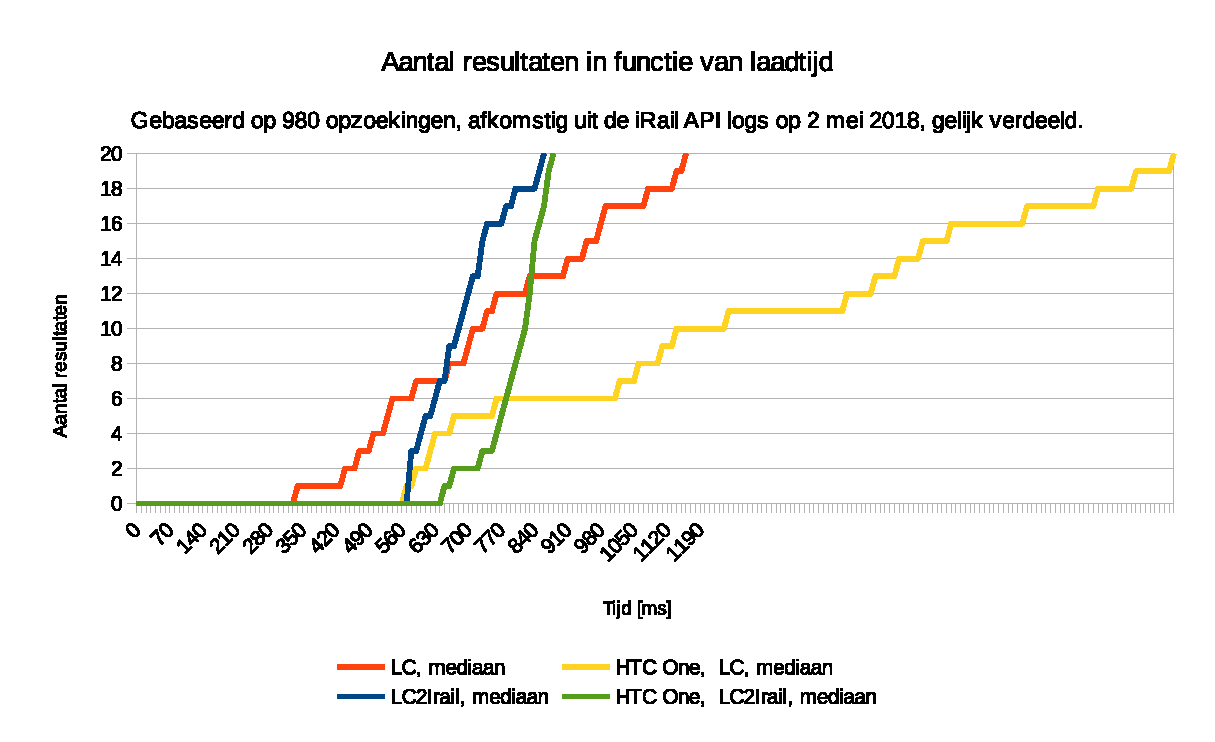
\includegraphics[width=.50\textwidth]{images/dief_liveboards_gemiddeld.eps}
		\caption{\label{fig:liveboard} }
	\end{center}
\end{figure}

Taking a look at the distributions of the loading times for the tenth results, visible in figure~\ref{fig:liveboardboxplot}, it is confirmed again that LC2Irail performs the same on both devices. This forms a contrast with Linked Connections, which has a significantly larger distribution of loading times on the HTC One. While the differences between the median response time of Linked Connections on the HTC 10 and LC2Irail on both devices can't be distinguished by end users %TODO: CITATION NEEDED
there is a clear difference with the median of Linked Connections on the HTC One.

\begin{figure}[ht]
	\begin{center}
		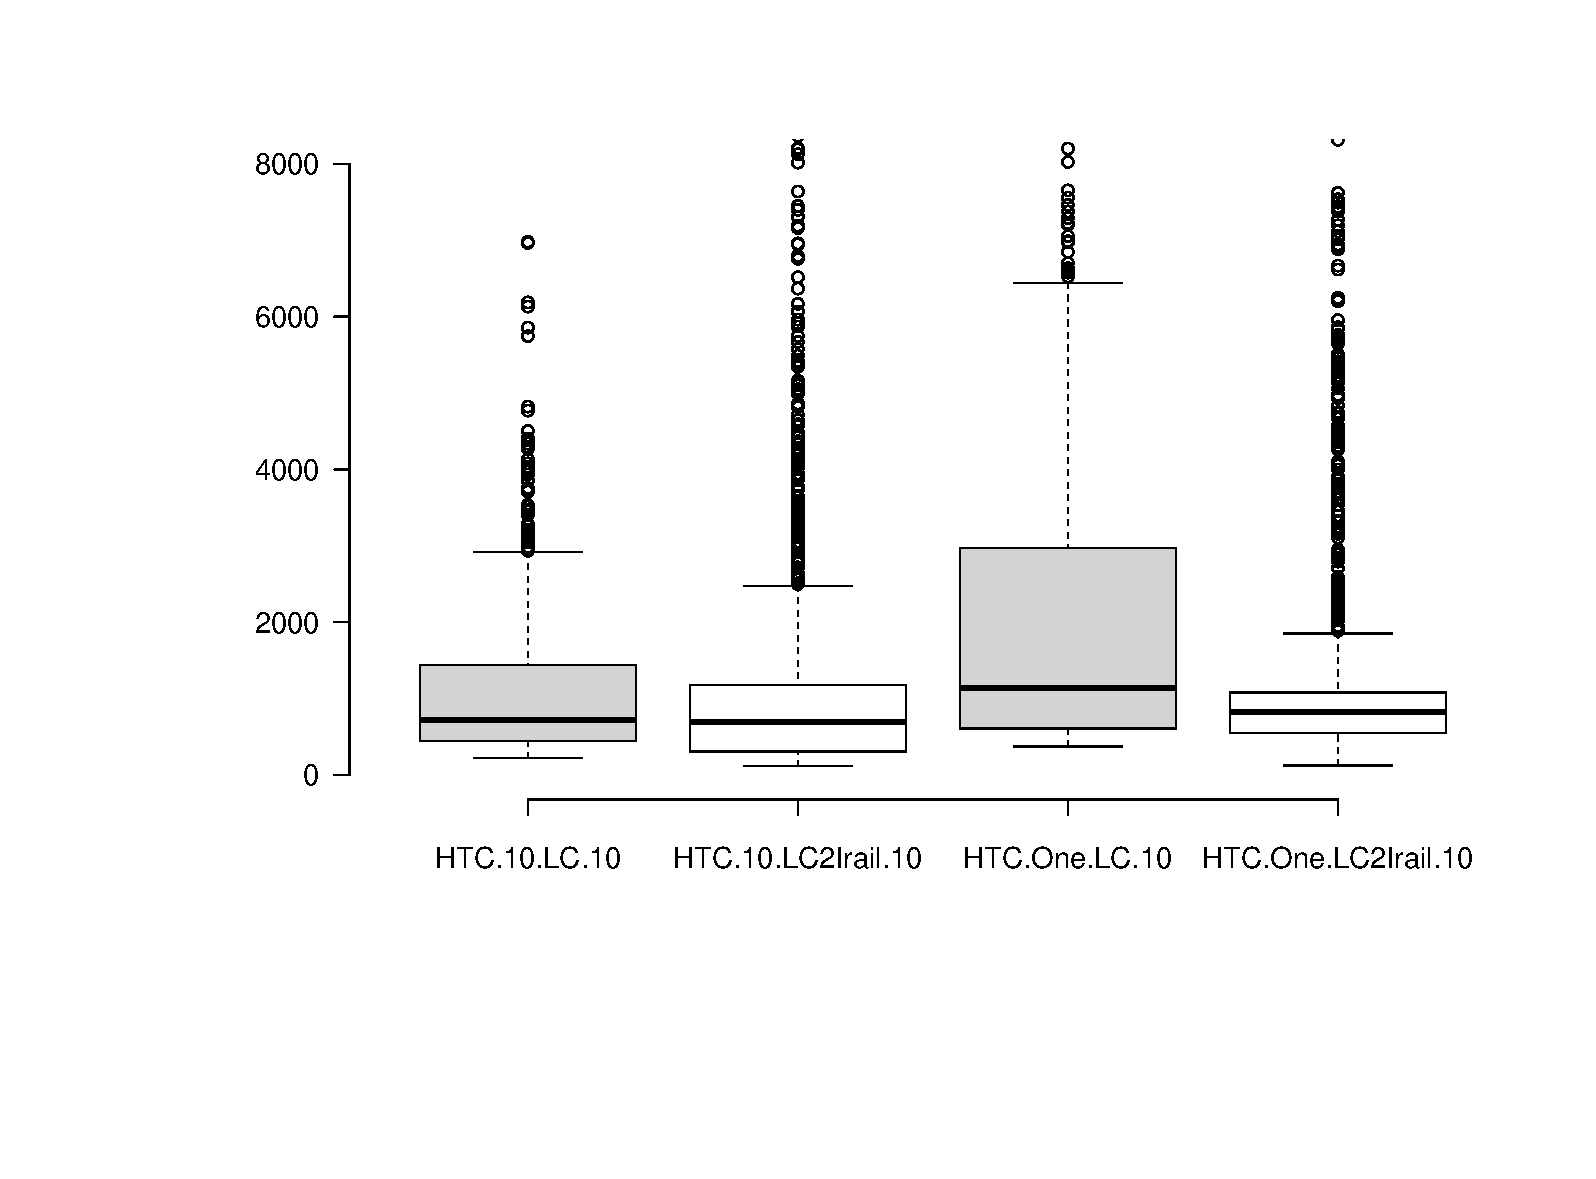
\includegraphics[trim=3cm 4cm 0 0, width=.50\textwidth]{images/boxplot_liveboards_10.eps}
		\caption{\label{fig:liveboardboxplot} }
	\end{center}
\end{figure}

When looking at the incremental results for routes, visible in figure~\ref{fig:route}, this difference between devices becomes even more visible. Linked Connections loads over 2 times faster on the HTC 10 compared to the HTC One. As a result, LC2Irail performs significantly worse than LC2Irail on the HTC One, even though Linked Connections performs better than LC2Irail on the modern HTC 10. LC2Irail performs again about the same on both devices.  This data type relies heavily on the Connection Scan Algorithm, which makes it even more surprising to see that Linked Connections on the HTC 10 is faster than the server. This is also a possible reason for the string discrepancy between loading times of Linked Connections on both devices.

\begin{figure}[ht]
	\begin{center}
		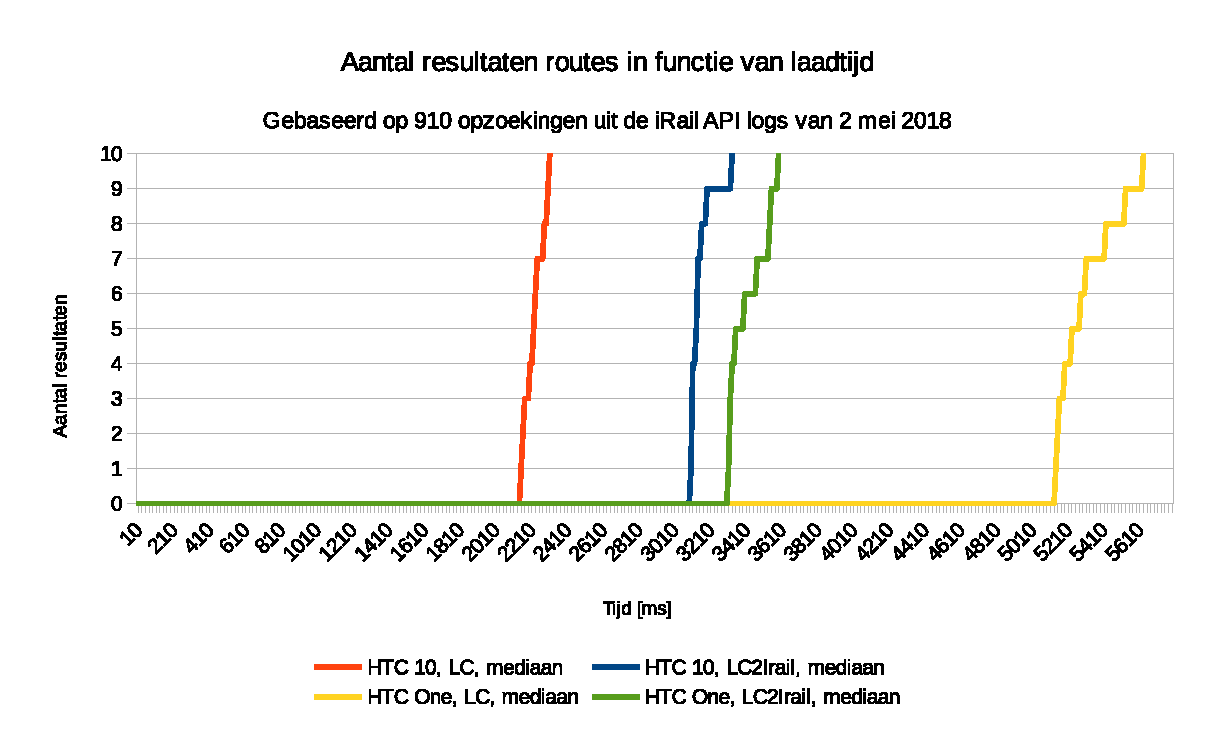
\includegraphics[width=.50\textwidth]{images/dief_routes_gemiddeld.eps}
		\caption{\label{fig:route} }
	\end{center}
\end{figure}

When the distributions for routes are plotted, shown in figure~\ref{fig:routebox}, this performance difference between devices becomes even more clear. The performance of LC2Irail for the tenth result sits in between the performance of Linked Connection on the HTC 10 and the HTC One. The differences between the medians and third quartiles are over one second. When it comes to the loading of results, this will impact the user experience in a negative way.

\begin{figure}[ht]
	\begin{center}
		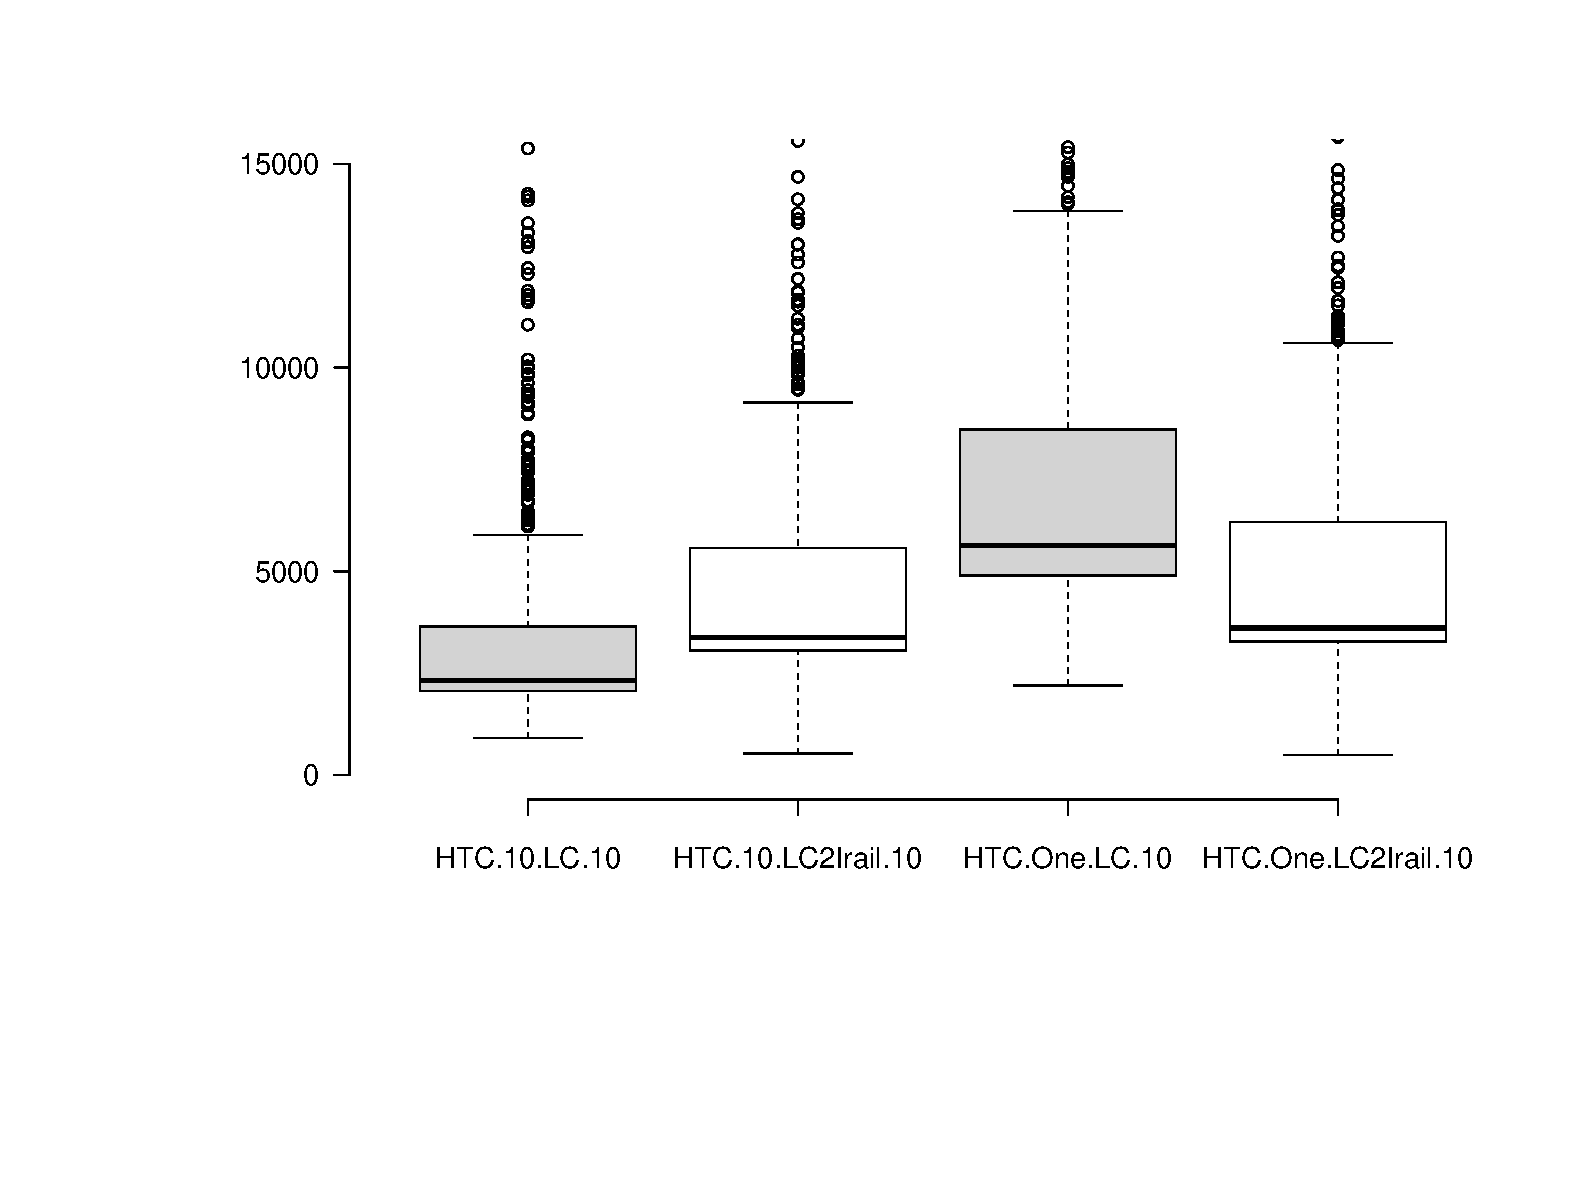
\includegraphics[trim=3cm 4cm 0 0, width=.50\textwidth]{images/boxplot_routes_10.eps}
		\caption{\label{fig:routebox} }
	\end{center}
\end{figure}

Vehicles, the last type of data, are special compared to the previous two. Every vehicle trip is considered to be one atomic result, therefore incremental results are not supported for this data type. When looking at the distribution of the loading times, as can be seen in figure \ref{fig:vehicle}, it becomes clear that vehicles take a long time to load, even though there are no complex algorithms needed. This data type needs a lot of data, however. LC2Irail, which has quick access to the data, performs a lot better here. Again, it performs consistently between devices, whereas Linked Connections needs two times as much time on the HTC One, compared to Linked Connections on the HTC 10.

\begin{figure}[ht]
	\begin{center}
		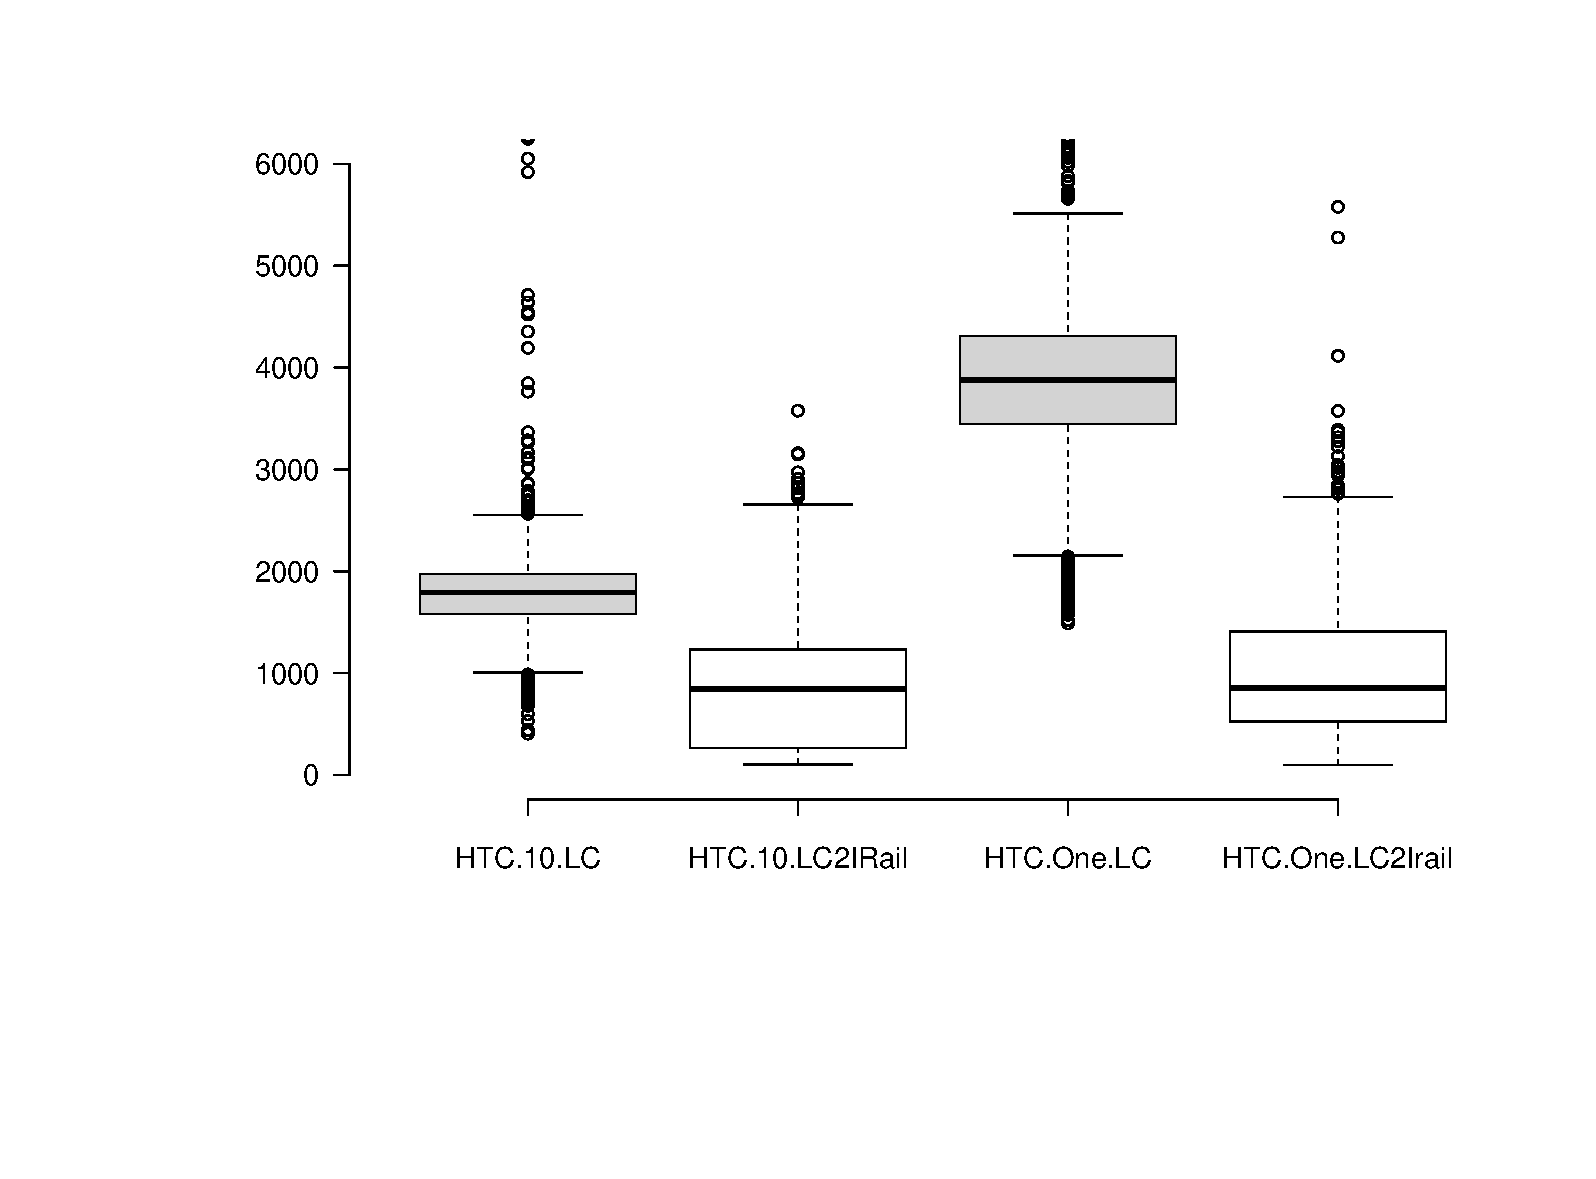
\includegraphics[trim=3cm 4cm 0 0, width=.50\textwidth]{images/boxplot_vehicles.eps}
		\caption{\label{fig:vehicle} }
	\end{center}
\end{figure}

Not only the data type and device affect the performance, but the exact query is of importance too. Calm stations, long routes, or vehicles with a long trip take longer to load compared to busy stations, short routes or vehicles with a short trip. The time to load a number of results is directly related to the timespan in which the results can be found. When a larger timespan needs to be evaluated, the results will take longer to load.

The measured results seem to match the user experienced performance. This can be seen in \ref{fig:choices}. While quite some users still find Linked Connections faster for departures, less people choose Linked Connections for routes, and even less choose Linked Connections for vehicles. However, when users are asked to not only judge by the performance, but to also take additional features like offline access into account, a majority of the users who previously chose for LC2Irail changes their mind and chooses Linked Connections. Features like incremental results don't seem to improve the user-perceived performance -- users keep waiting for all results to load before they start processing the results.

\begin{figure}[ht]
	\begin{center}
		\includegraphics[width=.40\textwidth]{images/alluvial_user_choice.eps}
		\caption{\label{fig:choices} }
	\end{center}
\end{figure}

\section{Discussion}

LC2Irail is a perfect reference API. The performance is consistent across devices, and users are overwhelmingly positive over the performance. Consistent good performance, with a small spread of the user-perceived performance, is the goal of every application. Linked Connections seems unable to offer this. The user perceived performance depends heavily on the use device, the type of data which was requested, and on the exact query. Both measured performance and user-perceived performance are spread out, ranging from slower than LC2Irail to faster than LC2Irail, and from perceived quite slow to perceived extremely fast. It seems there is definitely potential in this technique, but heavy resource requirements are holding it back on older devices. 

The difference between both Linked Connections implementations is an extremely important indicator. This difference shows that the performance of Linked Connections does not only depend on the device, data type and query, but also on the details of the implementation. When the parsing of both implementations is traced, the implementation based on \emph{LoganSquare} is about two times slower than the original implementation, requiring 200 milliseconds to parse a single Linked Connections page, compared to 100 milliseconds when using the \emph{org.json} parser. This is opposite to both benchmarks and user-perceived performance. The key to this mystery is found in the \emph{Garbage Collection} (GC), ran by the Android \emph{Java Virtual Machine} (JVM). The first implementation creates a multiple of the String objects created by the second implementation. As String objects are immutable, creating too much of them or modifying them too much will trigger garbage collection, in which case the entire application is frozen as unreferenced objects are removed from the memory. Even further, the JVM garbage collection treshhold depends on the heap size, which is configured by the device manufacturer and correlates with the available RAM and screen properties. This means older or cheaper devices are penalized twice: slower hardware means Linked Connections algorithms and GC take more time, while GC will be needed more often as the device has less memory.

Knowing now the importance of an efficient implementation on all levels, it is possible to reimplement the Linked Connections client while removing or reducing the usage of Strings. This might lead to further performance improvements, potentially bringing the performance on older or cheaper devices up to par with performance on more powerful devices. Still, this forms a disadvantage for Linked Connections. Developers looking to implement this might not have the necessary (background) knowledge to optimize their implementation this thorough, or they might not have the time. This could form a barrier for adaption. 

Another important curiosity is the U-turn most people made when asked to choose their favorite implementation, based on everything, including speed and offline access. While more and more people lean to LC2Irail depending on the endpoint, as can be seen in figure \ref{fig:choices}, offline access seems to convince over half of the people picking LC2Irail to switch to Linked Connections. This can be explained by the general discontent regarding mobile network coverage while travelling by train, and people not having access to mobile data, or being affraid of using too much.

Parameters like data usage depend heavily on the implementation. Various optimizations are possible to reduce this, with offline access reducing this to zero.

A last important note is the performance after mass adoption. While the RPC API will suffer from reduced performance under high load, Linked Connections provides better performance as load increases. This means the Linked Connections results will only improve, while the performance of the RPC API can only decline.
 
\section{Conclusion}
While the reference RPC API provides excellent results, Linked Connections offers a wide rang of performances depending on a lot of factors, sometimes performing better than this reference API, but often performing the same or worse. Users consistently perceive Linked Connections as slower, with only some outliers experiencing it faster. Performance heavily depends on the search, implementation and the users' device. This is a bad trait for an application, as the goal is to present a consistent experience across all devices. 

There is, however, a high chance that Linked Connections can be improved further by paying attention to implementation details. A second performance gain could be obtained by the use of various indices, reducing the overhead of retrieving pages without useful data. This could also be achieved by running the algorithms on cached data first, after which the used pages could be retrieved from the server in order to obtain realtime information. 

The performance of the route planning algorithm can be further optimized by first applying the Earliest Arrival Time algorithm, which will cache the required pages and determine the starting point where the Connection Scan Algorithm should start iterating over the pages. Search performance could also be improved by pre-loading data when it is highly likely the user will make a search. In this case it is no longer needed to retrieve the pages the moment the user confirms the search.

Another improvement could be obtained by first running the algorithm on cached or pre-loaded data. These results could be shown while real-time data is loaded from the server, after which the real-time data could be appended to the first results.

The last performance improvement could be achieved by keeping recently used pages in memory, thus reducing the amount of garbage, as it is likely that the next search will require data from the same page as the previous page. In reality, this might not be feasible due to constraints on the available memory. All performance improvements should take the device properties into account, as a device with limited RAM might be better off using a cache in the flash memory.
\nocite{*}
\bibliographystyle{phdsymp}
%%%%%\bibliography{bib-file} % commented if *.bbl file included, as
%%%%%see below


%%%%%%%%%%%%%%%%% BIBLIOGRAPHY IN THE LaTeX file !!!!! %%%%%%%%%%%%%%%%%%%%%%%%
%% This is nothing else than the phdsymp_sample2e.bbl file that you would%%
%% obtain with BibTeX: you do not need to send around the *.bbl file    
%%
%%---------------------------------------------------------------------------%%
%
\begin{thebibliography}{1}
\bibitem{colpaert17}
\bibitem{fielding99}
\bibitem{avila11}
\bibitem{verborgh16}
\end{thebibliography}
%
%%---------------------------------------------------------------------------%%

\end{document}

%%%%%%%%%%%%%%%%%%%%% End of phdsymp_sample2e.tex %%%%%%%%%%%%%%%%%%%%%%%%%%%
